
In this section, we will provide detailed explanations of the methods, techniques, and procedures employed in our experiments. We will begin by discussing the data preprocessing steps, followed by an explanation of the training process. Finally, we will describe how we evaluated the performance of our models.

\subsection{Engineering For Machine Learning}
In order to streamline our experimental process and minimize effort, we focused on developing the training and preprocessing code in a way that allows for easy experimentation. We also utilized tools that enhance efficiency and reproducibility in the research process, reducing time-consuming tasks.
\medskip

We adopted the \texttt{zenml} framework to structure our training and preprocessing pipelines. This framework brings several advantages to our workflow.
One notable benefit is the promotion of modularity in the design of our pipelines. Each pipeline consists of individual steps, which enhances the code's modularity. By defining a series of functions with clear inputs and outputs, we ensure that each step can be easily understood and modified as needed. Moreover, the \texttt{zenml} web application offers a convenient way to monitor the status of our pipelines. This feature provides transparency and improves comprehension by providing insights into the outputs generated at each step.
\medskip

For experiment tracking we used the \texttt{MLFlow} framwork.
This makes it easy to track all metrics over all experiments.
We can even track and visualize metrics during training of the models.
With \texttt{MLFlow} it is also possible to compare different parameters that were used during training to experimentally find the best combinations.
In \texttt{MLFlow} we save each finished model as an artifact which can be directly served as a server endpoint to start providing end users access to our models.
\medskip

We used the pytorch lightning library as well. Using patterns such as the \texttt{DataModule} and {LightningModule} to accelerate the
research process. The \mintinline{python}|class LightningModule| can be used by a configurable \mintinline{python}|class Trainer| to create a training loop, this ensures that we do not have 
to manually handle backpropagation or updating parameters. Furthermore pytorch ligthning handles
switching from training devices automatically from for example \texttt{cpu} and \texttt{cuda} which solves a lot of overhead in a programmer trying to remember which device each Tensor is on.

We made use of the \texttt{typed-settings} library to allow cleanly structuring and validating settings for models.
This ensures that to train a new version of a model in most cases only adjustments to the configuration file needs to be done.
\texttt{typed-settings} supports passing settings through toml confiuration files (See listing \ref{lst:hello}), environment variables and command line options.

\begin{listing}
  \begin{minted}{toml}
    [model]
    name = "SAT2RAD_UNET"
    classes=8
    
    [model.input_size]
    height = 256
    width = 256
    channels = 12
    sequence_length = 8
    
    [model.output_size]
    height = 256
    width = 256
    channels = 1
    sequence_length = 1
    
    [model.unet]
    kernel_size = [3, 3]
    layers = 3
    filters = 64
    
    [model.training]
    max_epochs = 100
    class_weights = [
                0.01081153,
                0.13732371,
                0.13895907,
                0.1416087,
                0.14272867,
                0.14285409,
                0.14285709,
                0.14285714,
            ]
    metrics = [
        'acc',
        'precision',
        'recall',
        'exact',
        'f1', 
        'jaccard'
    ]
    
    [mlflow]
    experiment_name = "sat2rad_unet"
    experiment_tracker = "Infoplaza MLFlow"
    
    
    [visualize]
    output_dir = '../../../../../logs/'
  \end{minted}
  \caption{toml configuration file for U-Net Model.}
  \label{lst:hello}
\end{listing}

\subsection{Data Preprocessing}

For the preprocessing of data we created a pipeline which distinguishes between satellite images and radar images to preprocess each following their own needs (See figure \ref{fig:preprocessing}).

The pipeline begins by obtaining all necessary files, from a remote storage bucket.
This is done by the \mintinline{python}|class BucketService()| which uses the \texttt{boto3}
library to interface with the bucket and downloads files in the required date ranges. In total we downloaded \texttt{3332} satellite files and \texttt{103348} radar files, this covers
all data from March 1st 2023 until April 5th 2023. This requires \texttt{387.6} Gigabytes of storage for only the preprocessed data.

In the case of satellite data, the obtained files are in compressed in zip files. The pipeline handles the extraction of these files deleting any files which are not needed along the way to ease the storage requirements.
Then we \textit{reproject} the satellite images using the \texttt{satpy} package. This downsampling is done by a combination of cropping and interpolation via a nearest-neihbor alorithm.

By reprojecting we reduce the dimensions of each satellite image to \texttt{256 x 256} pixels from it's original dimensions of (3712, 3712).
Via the reprojection we also obtain only the geographical area of interest, specified by the coordinates for the lower corner \texttt{(50°0'0"N 0°0'0"E)} and the upper corner \texttt{(55°0'0"N 10°0'0"E)} of the region, this gives us
the area centered on the netherlands with other bordering countries see figure 8.
Additionally the projection is matched between the satellite image and radar image.
After reprojecting we perform a \textit{statistics} step where we aggregate the dataset by finding the minimum and maximum values for each channel.
The statistics are necessary for the next step which is normalization. During the normalization step we perform the \textit{Min-Max} Normalization (equation 1).

\begin{equation}
  x_{normalized} = \frac{x-min_{\bar{x}}}{max_{\bar{x}}-min_{\bar{x}}}
\end{equation}

After finalizing the normalization step we sample an image from the dataset which is visualized to check for errors in the pipeline.

The radar pipeline begins with the downloading of radar files in the form of \texttt{h5} files. The collected files are each converted to decibels relative to Z (dBZ) from their previous unit.

\begin{equation}
  dBZ(x) = x \cdot 0.5 - 32
\end{equation}

The preprocessing pipeline then splits into two, one step will normalize values between 0 and 1 using \textit{Min-Max} normalization and the other step will use levels of \textit{dBZ} to create discrete ranges of precipitation to use as classes during training.
Finally the current images in the pipeline are resized using the nearest neighbor algorithm, to avoid changing the values with bilinear interpolation.
Next identically to the satellite pipeline we sample and visualize a radar image for verification purposes.


\begin{figure}
  \centering
  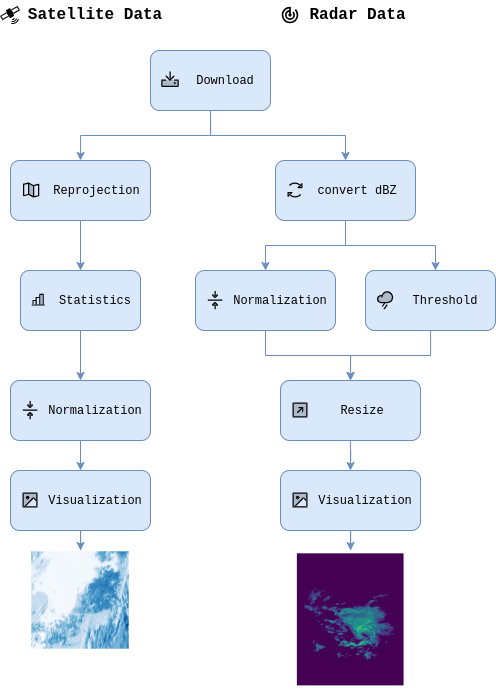
\includegraphics[width=225pt]{./images/prepro.png}
  \caption{Data Preprocessing Pipeline: Satellite Data and Radar data preprocessed separately}
  \Description{Satellite Image of the earth}
  \label{fig:preprocessing}
\end{figure}

\subsection{Model Training}
In order to build and train our models we worked with pytorch. We used pytorch lightning to provide a higher level interface to speed up the research process. To track our experiments we connected pytorch ligthning to mlflow, using MlFlow we can log metrics, artifacts produced during training while keeping track of the used parameters during that training run.
To create pipelines for preprocessing and training, we used the \texttt{zenml} library.

We created 4 different datasets for our research. These datasets result from the combination of sliding and sequential datasets with class and regression datasets.
We implemented these datasets as subclasses of pytorch vision datasets. We also created time based utility functions to align the start and ending times of satellite data and radar data, such that when data is split based on training, validation and testing percentages, data is still in the same temporal range. Keeping in mind that the radar data has a different resolution and is received at a different strides.

\subsection{Performance Evaluation}

Different metrics were used for the regression and the classification.

Classification evaluation metrics:
\begin{enumerate}
  \item Precision
  \item Accuracy
  \item Recall
  \item Exact Match
  \item F1 Score
  \item Jaccard Index
\end{enumerate}


\begin{equation}
  Precision = \frac{TP}{TP + FP}
\end{equation}

\begin{equation}
  Accuracy = \frac{TP+ TN}{TP + FP + TN + FN}
\end{equation}

\begin{equation}
  Recall = \frac{TP}{TP + FN}
\end{equation}

\begin{equation}
  F1Score = \frac{TP}{TP + \frac{1}{2}(FP + FN)}
\end{equation}

\begin{equation}
  Jaccard Index = \frac{TP}{TP + FP + FN}
\end{equation}

Regression Evaluation Metrics
\begin{equation}
  MSE = \frac{\sum (\hat{y_i} -y_i)^2}{n}
\end{equation}

\begin{equation}
MAE = \frac{\sum |\hat{y_i} -y_i|}{n}
\end{equation}

\begin{equation}
RMSE = \sqrt{\frac{\sum (\hat{y_i} -y_i)^2}{n}}
\end{equation}

Additional metrics come from the study \cite{shi2017deep}, where the authors created \textit{B-MSE} and \textit{B-MAE} due to the fact that the frequencies of different rainfall levels are imbalanced. Models trained with conventional \textit{MSE} or \textit{MAE} are biased towards predicting low amounts of precipitation. This can be solved with a loss function that weights the higher precipitation more strongly. The weighting function \textit{w} can be found in the study as well.

\begin{equation}
BMSE = \frac{\sum w(\hat{y_i}) \cdot (\hat{y_i} -y_i)^2}{n}
\end{equation}

\begin{equation}
BMAE = \frac{\sum w(\hat{y_i})  \cdot (\hat{y_i} -y_i)^2}{n}
\end{equation}
